\section{Method}
\label{section:method}
\subsection{Methodology}
The LSM6DSO sensor integrates both a gyroscope and an accelerometer, allowing it to measure both angular velocity and linear acceleration \cite{sensor}. The accelerometer has difficulties maintaining accuracy over short rapid movements, introducing noise to its measurement. And for the gyroscope, it tracks rotational motion but tends to drift due to the accumulation of small errors in each measurement. So to rely solely on one of the sensors makes it difficult to accurately estimate orientation.

To combat this flaw, a \textbf{Complementary filter} will be used to combine the strengths of both sensors\cite{Complementary}. These filters fuse the data, compensating for the weaknesses of each: the gyroscope drift is corrected by the accelerometer, and the accelerometer noise is smoothed by the gyroscope. This yields a more stable and accurate estimate of the sensor's orientation, which then can be used to interpret specific hand positions or gestures used in sign language.

\subsection{Hardware}
A simple hardware setup was used, consisting of an LSM6DSO sensor connected to a Raspberry Pi Zero 2 W board \cite{Rasp}. This configuration enables real-time acquisition of inertial measurements, while being small and light enough to enable future integration into wearable form factors. 

\subsection{Software}
The software was developed in Python as it is one of the most common programs used for raspberry pi coding \cite{Rasp_python}. And one of the main reason for it is due to it's large selection of libraries. One of them is the I2C protocol that will be used for for the communication between the sensor and Raspberry.

To enable parallel development of hardware and software, test data simulating sensor readings were first generated and used in place of live data. A simple Python code modeled a single finger starting in a reference position(fully extended), to being bent 45 degrees, then returns back to the reference position. With a known movement the measured value could be understood better and conclusions drawn about the Complementary filters performance could be evaluated. The simulated data are output as comma-separated values in the order:"accel-x, accel-y, accel-z, gyro-x, gyro-y, gyro-z".

From these raw values, pitch and roll angles were calculated independently using the accelerometer and gyroscope. The accelerometer-derived angles were calculated using trigonometric functions, based on the ratio of acceleration in each axis, while the gyroscope-derived angles were obtained by integrating the angular velocity over time. Both pitch and roll are calculated using similar mathematical expressions, with only a change in which axes are involved. For clarity and to avoid redundancy, only the pitch formulas are presented below.

For the accelerometer-based estimation, the pitch angle is computed using the $x$-axis acceleration and the combined magnitude of the $y$- and $z$-axes. Roll follows the same structure but switches to using the $y$-axis in the numerator. See equation~\ref{eq:accel_pitch}.

For the gyroscope-based estimation, pitch is calculated by integrating the angular velocity around the $x$-axis, while roll uses the angular velocity around the $y$-axis. See equation~\ref{eq:gyro_pitch}.

As mentioned in the methodology subsection, each part of the sensor has limitations that will be mitigated by implementing a Complementary filter. This filter combines both data sources by weighting them according to their respective reliability: the short-term precision of the gyroscope and the long-term stability of the accelerometer. The resulting output provides a more accurate and stable estimate of the sensor's orientation, specifically the pitch (vertical bending) and roll (side tilt) of the finger. See equation~\ref{eq:complementary_pitch}.

\begin{equation}
\theta_{\text{pitch, accel}} = \arctan\left( \frac{a_x}{\sqrt{a_y^2 + a_z^2}} \right)
\label{eq:accel_pitch}
\end{equation}

\begin{equation}
\theta_{\text{pitch, gyro}} = \theta_{\text{filtered, pitch}} + \omega_x \cdot \Delta t
\label{eq:gyro_pitch}
\end{equation}

\begin{equation}
\theta_{\text{pitch,filt}} = \alpha \cdot (\theta_{\text{pitch,gyro}}) + (1 - \alpha) \cdot \theta_{\text{pitch,acc}}
\label{eq:complementary_pitch}
\end{equation}

\noindent
\textbf{Variable definitions:}
\begin{itemize}
    \item $\theta_{\text{pitch, accel}}$ – Estimated pitch angle from the accelerometer.
    \item $a_x, a_y, a_z$ – Acceleration values along the respective axes.
    \item $\theta_{\text{pitch, gyro}}$ – Estimated pitch angle from the gyroscope.
    \item $\theta_{\text{previous, pitch}}$ – Previously calculated pitch angle.
    \item $\omega_x$ – Angular velocity around the $x$-axis (in rad/s).
    \item $\Delta t$ – Time elapsed since the previous measurement (in seconds).
    \item $\alpha $ – Weight constant (0.98 was used, commonly between 0.9 and 0.98).
\end{itemize}

The code process can be summarized in the following steps:
\begin{figure}[H]
    \centering
    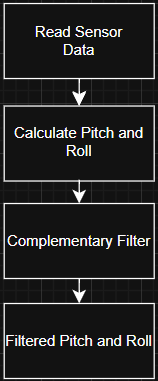
\includegraphics[width=0.15\textwidth]{images/FlowChart.png}
    \caption{Overview of the software flowchart. The chart outlines the program's execution from simulated sensor input to orientation estimation using sensor fusion.}
    \label{fig:software_flowchart}
\end{figure}